\chapter{Generative AI Disclosure}
\label{app:ai-disclosure}

In accordance with DTU's guidelines on the use of generative AI tools in
academic work, the following AI-assisted tools were used during the
preparation of this thesis.

\textbf{Claude Code (Anthropic)} was used as a coding assistant during
the implementation of the evaluation pipeline, HPC job scripts, and data
processing scripts. Generated code was reviewed, tested, and modified
before use. No generated code was submitted without verification against
expected outputs.

\textbf{Claude (Anthropic, claude.ai)} was used as a writing assistant
to produce draft text for thesis sections. \textbf{Codex in ChatGPT
(OpenAI)} was also used as a writing assistant for revising thesis prose,
improving structure, and clarifying explanations. All drafted or revised
text was reviewed, modified, and rewritten in the author's own voice before
inclusion. The author is responsible for all factual claims, experimental
results, and interpretations presented in this thesis.

No AI tool was used to generate experimental data, benchmark results,
or citations. All numerical results reported in this thesis were produced
by running experiments on the DTU HPC cluster and collected by the author.

AI tools are not listed as authors or co-authors of this work, in
accordance with the Vancouver Convention as adopted by
DTU~\cite{ICMJE2020vancouver}.

\chapter{Hyperparameters and Training Details}
\label{app:hyperparameters}

Table~\ref{tab:lora-hyperparams} lists the hyperparameters used for
LoRA fine-tuning in all training configurations.

\begin{table}[ht]
\centering
\caption{LoRA fine-tuning hyperparameters for all training configurations.}
\label{tab:lora-hyperparams}
\begin{tabular}{ll}
\toprule
Parameter & Value \\
\midrule
Base model & \texttt{Qwen/Qwen2.5-7B-Instruct} \\
Dataset & \texttt{Salesforce/xlam-function-calling-60k} \\
Training examples & 54{,}000 \\
Validation examples & 6{,}000 \\
LoRA rank & 16 \\
LoRA alpha & 32 \\
Target modules & \texttt{q\_proj, v\_proj} \\
Dropout & 0.05 \\
Epochs & 2 \\
Batch size & 4 \\
Gradient accumulation steps & 4 \\
Learning rate & $2 \times 10^{-4}$ \\
LR scheduler & cosine \\
Dtype & bfloat16 \\
Optimizer & AdamW \\
Max sequence length & 2048 \\
\bottomrule
\end{tabular}
\end{table}

Fig.~\ref{fig:lora-training-loss} shows the training loss for the two LoRA
adapters discussed in Section~\ref{sec:format-aligned}.

\begin{figure}[htbp]
\centering
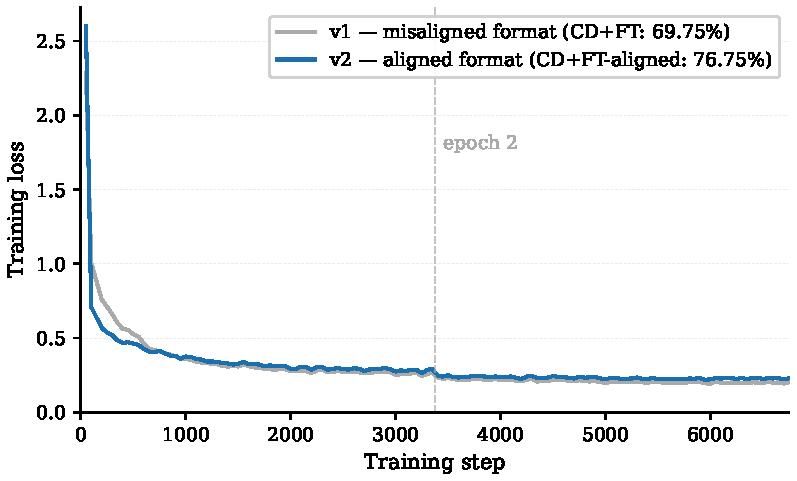
\includegraphics[width=0.65\textwidth]{pictures/figures/fig_lora_training_loss.pdf}
\caption{Training loss for the misaligned (v1) and format-aligned (v2) LoRA
         adapters over 6{,}750 steps (2 epochs on 54{,}000 xlam examples).
         Both runs converge to comparable loss values; the 7.0~pp accuracy
         difference between CD+FT and CD+FT-aligned is caused
         by the training output format, not by training quality.}
\label{fig:lora-training-loss}
\end{figure}

\chapter{Full Benchmark Results}
\label{app:benchmark-results}

Table~\ref{tab:full-results} reports the complete per-configuration results
on BFCL~v4 \texttt{simple\_python} (400 test cases).

\begin{table}[ht]
\centering
\caption{Full BFCL~v4 \texttt{simple\_python} AST accuracy results across all
configurations evaluated in this thesis. Config~B reports the strict
whole-completion-parse floor; the no-guided rows (RAG-ng, PE-ng, ITC-ng,
FT-only, FT-aligned-ng) use the lenient first-complete-object parser, matching
the isolation arm in Section~\ref{sec:technique-isolation}
(Tables~\ref{tab:isolation} and~\ref{tab:cd-contribution}). The two parse
criteria are defined in Section~\ref{sec:baseline-def}.}
\label{tab:full-results}
\resizebox{\textwidth}{!}{%
\begin{tabular}{llrrl}
\toprule
Config & Description & Correct & Accuracy ($\uparrow$) & Delta vs CD \\
\midrule
B           & No constrained decoding           & 6/400   & 1.50\%  & $-71.25$~pp \\
B-template  & Native template, free generation  & 384/400 & 96.00\% & $+23.25$~pp \\
PE      & CD + few-shot (3 examples)        & 281/400 & 70.25\% & $-2.50$~pp  \\
CD      & Constrained decoding              & 291/400 & 72.75\% & baseline    \\
CD+Q    & CD + AWQ INT4                     & 289/400 & 72.25\% & $-0.50$~pp  \\
CD+Q+ITC & CD+Q + chain-of-thought         & 262/400 & 65.50\% & $-7.25$~pp  \\
CD+Q+RAG & CD+Q + FAISS top-5              & 191/400 & 47.75\% & $-25.00$~pp \\
RAG-ng  & Retrieval, no CD                  & 208/400 & 52.00\% & $-20.75$~pp \\
PE-ng   & Few-shot, no CD                   & 236/400 & 59.00\% & $-13.75$~pp \\
ITC-ng  & Chain-of-thought, no CD           & 225/400 & 56.25\% & $-16.50$~pp \\
FT-only & LoRA merged, no CD               & 212/400 & 53.00\% & $-19.75$~pp \\
CD+FT   & CD + LoRA merged (v1)            & 279/400 & 69.75\% & $-3.00$~pp  \\
FT-aligned-ng & Format-aligned LoRA, no CD   & 164/400 & 41.00\% & $-31.75$~pp \\
CD+FT-aligned   & CD + format-aligned LoRA             & 307/400 & 76.75\% & $+4.00$~pp  \\
CD+Q+FT-aligned & CD + AWQ INT4 + format-aligned LoRA  & 297/400 & 74.25\% & $+1.50$~pp  \\
\textbf{CD+schema} & \textbf{CD + schema-enriched prompt} & \textbf{356/400} & \textbf{89.00\%} & $\mathbf{+16.25}$~\textbf{pp} \\
\bottomrule
\end{tabular}%
}
\end{table}

\chapter{Updated Project Plan: Deviations from the Original Plan}
\label{app:project-plan-update}

This appendix updates the project plan submitted at the start of the
project, as required for hand-in. It records the parts of the project
that changed significantly from the original plan; the original
motivation, research question, and time plan are otherwise unchanged.

\section{Scope and framing}

The original plan positioned constrained decoding (CD) as the core
contribution, supported by a set of complementary efficiency techniques
(quantization, LoRA fine-tuning, retrieval-augmented generation, and
possibly knowledge distillation). The final thesis keeps CD as the core,
but the framing shifted to expressing each technique as a candidate for
\emph{expanding the boundary of a cascade LLM architecture}, i.e.\ how
far a small model can be pushed before a request must be escalated to a
larger model.

\section{Changes to the experimental program}

The most significant deviation concerns the role of the complementary
techniques. The original plan treated them as additive improvements on
top of CD. The experiments showed the opposite for several of them:

\begin{itemize}
  \item Retrieval-augmented generation reduced accuracy substantially
        ($-25$~pp relative to plain CD) rather than improving it.
  \item In-context chain-of-thought (ITC) also reduced accuracy
        ($-7.25$~pp).
  \item AWQ INT4 quantization was approximately neutral ($-0.50$~pp),
        confirming it as a low-cost compression option rather than an
        accuracy lever.
  \item LoRA fine-tuning helped only modestly and only in combination
        with CD (format-aligned LoRA: $+4.00$~pp), and collapsed to near
        zero accuracy without guided decoding.
\end{itemize}

Knowledge distillation, listed in the original plan as an optional
alternative, was not pursued; it was de-scoped to keep the analysis
focused on the techniques above, as anticipated by the risk-mitigation
note in the original plan.

The strongest configuration in the final thesis, \texttt{CD+schema}
(a schema-enriched argument-extraction prompt, $+16.25$~pp over plain
CD), was not part of the original plan. It emerged from analysing the
failure modes observed during the constrained-decoding experiments and
became a central result.

\section{Time plan}

% TODO (author): in your own words, note any timing deviations from the
% Gantt chart in the original plan, e.g. whether the "Exploration of
% alternative efficiency techniques" phase ran longer/shorter than
% planned, and how report writing overlapped with experimentation.

\chapter{Self-Evaluation of the Project Process}
\label{app:self-evaluation}

% TODO (author): this chapter is a required, personal reflection on how
% the project went. Write it in your own voice. Use the prompts below as
% a guide and delete them once written. This is a solo thesis, so the
% group-work and company prompts from the DTU hand-in guidelines do not
% apply.

% - Did you follow the time plan? Which phases ran to schedule and which
%   slipped? What caused the slips (e.g. HPC queue times, .venv/uv sync
%   races, baseline parser drift requiring reruns)?
%
% - What problems did you encounter during the project, and how did you
%   resolve them? (e.g. shared-NFS environment corruption, stale
%   aggregate score files vs. per-run source of truth, no-guided baseline
%   parser sensitivity inverting headline numbers.)
%
% - What would you do differently with hindsight? (e.g. lock the parser
%   definition earlier, pre-sync the environment before parallel jobs.)
%
% - What did you learn from the process, beyond the technical results?
